\documentclass[aps,twocolumn,secnumarabic,nobalancelastpage,amsmath,amssymb,nofootinbib]{revtex4-1}
\usepackage{graphics}      
\usepackage{graphicx}      
\usepackage{longtable}     
\usepackage{url}          
\usepackage{bm}           
\usepackage[utf8]{inputenc}
\usepackage[dvipsnames]{xcolor}
\usepackage{tikz}


\begin{document}
	\title			{P\'endulo casero amortiguado y sus caracter\'isticas en la din\'amica del sistema}
	\author			{Carlos Cardinale}	
	\email			{carlos.cardinale@ucr.ac.cr}
	\affiliation	{Escuela de Física, Universidad de Costa Rica}
	%\date			{}
	
		\begin{abstract}
			Se estudia el sistema del p\'endulo amortiguado y se demuestra que su din\'amica no es estrictamente ca\'otica. Este sistema si comparte caracteristicas claves de un movimiento ca\'otico pero carece de variables din\'amicas para poder considerarlo ca\'otico. La energ\'ia siempre tiene mayor decaimiento en los primero periodos y la soluci\'on de Runge-Kutta para el diagrama de fase del movimiento completo est\'a dada y discutida en la investigaci\'on.       	
		\end{abstract}
	
	\maketitle
	     	    
	\section{Introducci\'on}
		El movimiento de un p\'endulo para \'angulos pequeños, movimiento arm\'onico simple, es de lo m\'as estudiado en la f\'isica. Aparece muchas veces en las teor\'ias de investigaci\'on desde la mec\'anica cl\'asica hasta la cu\'antica y por eso su estudio ha abarcado gran importancia. La soluci\'on para el movimiento de cualquier \'angulo (de $-\pi$ a $\pi$) no es exacta, tampoco, al introducir la fuerzas no conservativas; cosa que se tomar\'a en cuenta en el experimento. \\ 
		\indent Para solucionar tal movimiento generalizado es indispensable saber de m\'etodos num\'ericos y su respectiva programaci\'on computacional.  \\		
		%\indent El p\'endulo doble es otro sistema que su movimiento es interesante ya que es ca\'otico por si s\'olo y al introducir la fuerzas no conservativas el sistema puede tomar movimientos muy interesantes. Este sistema es evidentemente m\'as complejo. Su din\'amica puede ser simulada con algoritmos computacionales y su estudio ayuda a entender m\'as sobre sistemsa ca\'oticos y sobre sistemas ca\'oticos con fuerzas no conservativas.
		\indent Por lo tanto, se planea entender por completo el movimiento del p\'endulo simple 
		%y doble 
		como se da en la naturaleza. En otras palabras, 
		%ambos sistemas ser\'an estudiados 
		se estudia el p\'endulo simple sin sobre simplificar el movimiento y, en un principio, tomando en cuenta toda variable que afecte su din\'amica. Como por ejemplo, resistencia del aire o fricci\'on que se pueda dar en la oscilaci\'on. \\
		
		
		
		\subsection{Pregunta de Investigaci\'on}
			¿%Son naturalmente ca\'oticos los sistemas de el p\'endulo simple y el p\'endulo doble al agregarle fuerzas no conservativas al movimiento
			Es naturalmente ca\'otico el sistema de p\'endulo simple al agregarle fuerzas no conservativas, disipadoras, al movimiento?  
		\subsection{Objetivo General}
			Fortalecer las bases de m\'etodos num\'ericos, y programaci\'on cuando se estudian sistemas con soluciones no anal\'iticas. 
		\subsection{Objetivos Espec\'ificos}
			\begin{itemize}
				\item Crear un sistema de p\'endulo simple con materiales caseros que permitan el estudio detallado de su movimiento. %y doble con materiales caseros.
				\item Analizar datos, por medio de una aplicaci\'on m\'obil de alto nivel algor\'itmico, para la toma de fotos, con alta calidad, en cuadros por segundo.
				\item Demostrar que en la naturaleza hay sistemas complejos que su soluci\'on es posible solo con m\'etodos num\'ericos.
				\item Mostrar diagramas de fase para cada condici\'on inicial para determinar si el movimiento es ca\'otico. 
			\end{itemize}
				
	\section{antecedentes y Marco Te\'orico}
		El p\'endulo simple en $\mathbb{R}^2$, sin incluir fuerzas no conservativas, tiene energ\'ia cin\'etica igual a $\frac{1}{2}m(l{\dot{\theta}})^2$ con energ\'ia potencial de $-mglcos(\theta)$; donde $m, l, \theta, {\dot{\theta}}$ son la masa, longitud de la cuerda, el \'angulo de oscilaci\'on y la derivada del \'angulo con respecto al tiempo. El Hamiltoniano tiene la siguiente forma:	
		\begin{equation}
			H = p_\theta \dot{q}_\theta-L(\theta,t) = \frac{1}{2}\frac{p_\theta^2}{ml^2}-mglcos(\theta) 
			\label{HamiltonianoCon}
		\end{equation}
		\noindent donde $L(\theta,t)$ es el Lagrangiano, $p_\theta$ es el momentum generalizado y $t$ es el tiempo. El Hamiltoniano anterior es conservativo a no depender explicitamente del tiempo\cite{taylor2005classical}, y considerando solo \'angulos pequeños, se puede obtener la ecuaci\'on de movimiento:	
		\begin{equation}
			\ddot{\theta} + \omega^2\theta	= 0
		\end{equation}    	
		\noindent con $\omega^2=g/l$. Esta es una ecuaci\'on altamente conocida por ser la ecuaci\'on del movimiento arm\'onico simple\cite{morin2008introduction}. \\	
		%\indent Para el p\'endulo doble se tiene un caso similar solo que ahora con dos grados de libertad en total, uno m\'as comparado con el p\'endulo simple. La energ\'ia cin\'etica para el p\'endulo doble, considerando solo \'angulos pequeños, es igual a $\frac{1}{2}(m_1 + m_2)l_1^2\dot{\theta_1}^2 + m_2l_1l_2\dot{\theta_1}\dot{\theta_2} + \frac{1}{2}m_2l_2^2\dot{\theta_2}^2$; donde $m_1, m_2, l_1, l_2, \dot{\theta_1}, \dot{\theta_2}$, es la masa de una particula, la masa de la otra part\'icula, la longitud de la cuerda con respecto a la primera masa, la longitud de la cuerda con respecto de la primera masa a la segunda masa, la derivada del \'angulo de oscilaci\'on de la primera masa con respecto al tiempo y la derivada del \'angulo de la segunda masa con respecto al tiempo. La respectiva energ\'ia potencial del sistema es igual a $\frac{1}{2}(m_1 + m_2)gl_1\theta_1^2 + \frac{1}{2}m_2gl_2\theta_2^2$; donde $g$ es la aceleraci\'on de gravedad. Al tener dos grados de libertad se obtienen dos ecuaciones de movimiento independiente. Las ecuaciones calculadas son las siguientes: 
		%\begin{equation}
		%	(m_1 + m_2)l_1^2\ddot{\theta_1} + m_2l_1l_2\ddot{\theta_2} = -(m_1 %+ m_2)gl_1\theta_1
		%\end{equation} 
		%y 
		%\begin{equation}
		%	m_2l_1l_2\ddot{\theta_1} + m_2l_2^2\ddot{\theta_2} = %-m_2gl_2\theta_2.
		%\end{equation}
		%Estas dos ecuaciones podrian ser expresadas en matrices\cite{taylor2005classical}.\\
		%\indent Ahora a cada sistema se le agrega la fuerza de fricci\'on y adem\'as se toma en cuenta el movimiento para cualquier \'angulo entre 0 a $\pi$. Estas dos consideraciones que son indispensables al movimiento real de los pendulos complican bastante el c\'alculo anterior. En el caso del p\'endulo simple para cualquier \'angulo se tendr\'ia la misma energ\'ia cin\'enica y la misma energ\'ia potencial. Lo que cambia es la energ\'ia total ya que deja de ser conservativa. Debido a la fricci\'on la energ\'ia disminuye con respecto al tiempo. La ecuaci\'on de Hamilton del p\'endulo simple para este caso ser\'ia:
		\indent Ahora al sistema se le agrega las fuerzas no conservativas que son disipadoras de la energ\'ia y adem\'as se consideran \'angulos de 0 a $\pi$. Estas consideraciones complican m\'as el c\'alculo anterior. Entonces, para un \'angulo determinado lo que cambia es la energ\'ia despues de un tiempo ya que deja de ser conservativa. Esto entonces depende estrictamente de la posici\'on inicial del sistema\cite{galley2013classical}. Debido a la fricci\'on la energ\'ia disminuye con respecto al tiempo. La ecuaci\'on de Hamilton del p\'endulo simple para este caso ser\'ia:   
		\begin{equation}
			H'(\theta; p_\theta; t) = H^{(0)} + H^{(1)}.
			\label{EcuacionHamilton} 
		\end{equation}
		$H^{(0)}$ de la ecuaci\'on anterior es el Hamiltoniano constante en el tiempo calculado en la ecuaci\'on ($\ref{HamiltonianoCon}$), $H^{(1)}$ es el t\'ermino nuevo que aparece debido a la fuerza de fricci\'on en el nuevo Hamiltoniano, $H'$. $H^{(1)}$ es dependiente del tiempo y cuando $t\rightarrow\infty$ entonces $H'\rightarrow0$. Esto es esperado por el hecho que en la naturaleza todo p\'endulo deja de oscilar despu\'es de cierto tiempo. La ecuaci\'on del movimiento en t\'erminos generales del \'angulo, $\theta$, viene dada por:
		\begin{equation}
			\ddot{\theta} + f_1(\theta, t)\dot{\theta} + f_2(\theta, t) = 0
			\label{ecuacionMovimiento}
		\end{equation}
		
		\noindent La ecuaci\'on se estudiar\'a mas a fondo cuando se expliquen los resultados obtenidos por medio de m\'etodos num\'ericos como Runge-Kutta\cite{scheck2010mechanics}. $f_1$ y $f_2$ ser\'an entonces aproximados con m\'etodos num\'ericos. Las fuerzas disipativas pueden ser no lineales y tener una forma polinomial\cite{trueba2003generalized}. Solo se considera el t\'ermino lineal ya que de incluir m\'as t\'erminos en las fuerzas disipativas solo complica el sistema, pero no afecta en el cumplimiento de los objetivos planteados.   
	
		%\indent El sistema de doble p\'endulo al igual que el p\'endulo simple deja de oscilar cuando el tiempo es significativamente grande. La ecuaci\'on que se va a aproximar tiene la forma de:
		%\begin{equation}
		%	H''(\{\theta\}; \{p_\theta\}; t) = H^{(0)} + H^{(1)} + H^{(2)} 
		%\end{equation}   
		%donde el sub-indice dos est\'a para diferenciar del caso del pendulo simple. $H^{(1)}_2$ es el t\'ermino no conservativo proveniente de de la fuerza de fricci\'on de la primera masa y $H^{(2)}$ corresponde a lo mismo pero para la segunda masa. 
	
		\indent El diagrama de fase en este sistema no lineal puede ser graficado por computadora\cite{marion2013classical} una vez se tenga la energ\'ia potencial total aproximada experimentalmente. Para el caso del p\'endulo simple con un solo grado de libertad la ecuaci\'on tiene la forma siguiente:
		\begin{equation}
			\dot{\theta}(\theta) \propto \sqrt{E-U(\theta)}
		\end{equation} 
		El diagrama de fase adem\'as puede mostrar claramente el atractor del sistema. El atractor es un conjunto de puntos, o punto, en el diagrama de fases del cual la soluci\'on del sistema tiende a comportarse despu\'es de un tiempo largo\cite{goldstein1980classical}. El atractor para el p\'endulo simple amortiguado sin fuerzas impulsadas ser\'ia la posici\'on en el cual deje de oscilar por completo\cite{tel2006chaotic}. Este punto por lo general es el origen del sistema pero depende del marco de referencia. De cualquier modo, el diagrama de fase puede ser centralizado, cosa que se hace en el paper.       
		%\indent El p\'endulo doble con dos grados de libertad tendr\'ia dos diagramas de fase, uno por cada grado de libertad. La ecuaci\'on se expresa de la siguiente forma:
		%\begin{equation}
		%	\dot{\theta}_{1,2} \propto \sqrt{E-U(\theta_{1,2})}.
		%\end{equation} 
		%en la cual el sub-indice indica con respecto a que \'angulo se est\'a graficando.\\
		%\indent El p\'endulo doble es un sistema ca\'otico por lo tanto se espera que el diagrama de fase de una forma irregular que parezca que su movimiento es random, pero a\'un as\'i est\'a moderado por las restricciones dadas\cite{goldstein1980classical}. 
		   	
		       
	\section{Experimento}
		\subsection{Materiales}
			\begin{itemize}
				\item Cuerda de aproximadamente 10.15cm $\pm$ 0.2cm
				\item Una masa con peso aproximado de 1.8g $\pm$ 0.01g  
				\item Pl\'astico protector transparente
				\item C\'amara de video con capacidad de grabar video en alta definici\'on a c\'amara lenta de 32x(960 fps)
				\item Computadora
				\item Cron\'ometro
				\item Protractor
			\end{itemize}
		\subsection{Procedimiento y m\'etodos}
			%El experimento es constru\'ido con los materiales antes mencionados. Facilmente se pueden construir los dos sistemas que se desean estudiar. La forma conveniente de armar el equipo, con los materiales, es como se muestra en las figuras (FIG. 1 y FIG. 2).
			El experimento es constru\'ido con los materiales antes mencionados. Facilmente se pueden construir el sistema que se desea estudiar. La forma conveniente de armar el equipo, con los materiales, es como se muestra en la figura \ref{fig:esquemaExp}.
			\begin{figure}[!htb]
				\center{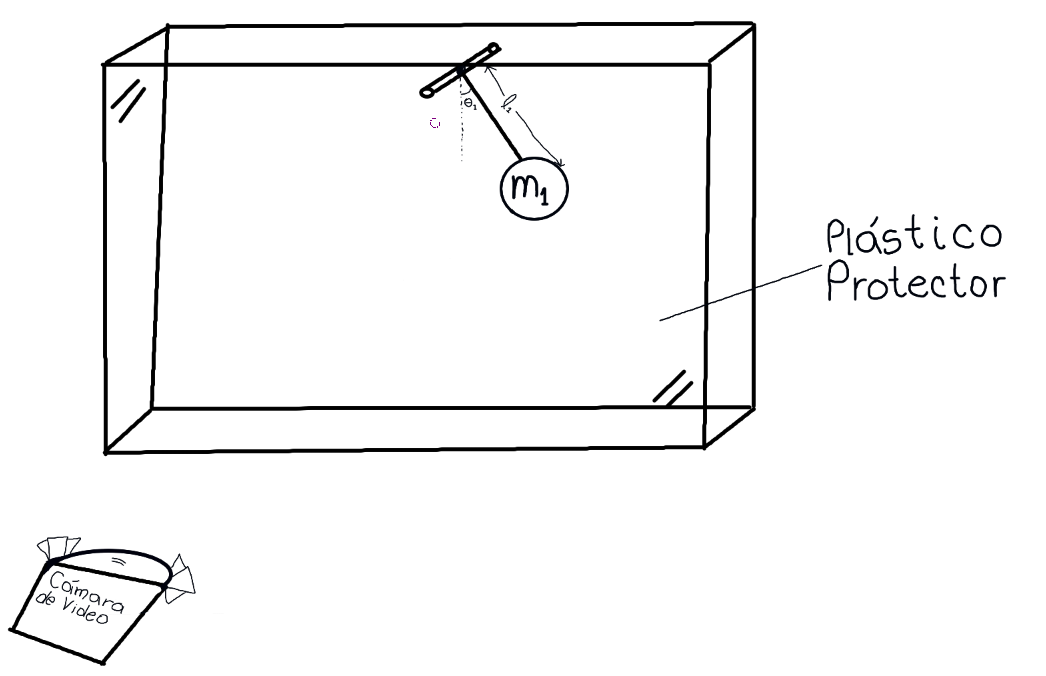
\includegraphics[width=8cm, height=5cm]
					{figura1MyPaper.png}}
				\caption{Esquema del experimento para el p\'endulo simple donde se muestra como es armado el equipo.}
				\label{fig:esquemaExp}
			\end{figure} 
			%\begin{figure}[!htb]
			%	\center{\includegraphics[width=8cm, height=5cm]
			%		{figura2MyPaper.png}}
			%	\caption{\label{fig:my-label} Esquema del experimento para el p\'endulo doble donde se muestra como es armado el equipo.}
			%\end{figure}  
		
			%Una vez armado el sistema de p\'endulo simple y doble, se explica paso a paso la manera de tomar los datos experimentales.
			Una vez armado el sistema de p\'endulo simple, se procede a explicar paso a paso la manera de tomar los datos experimentales.
			
			%\noindent\textbf{P\'endulo Simple}
			
			El procedimiento para el caso del p\'endulo simple es:
			\begin{enumerate}
				\item Toma de datos en el \'angulo de 30 grados.
				\item Toma de datos en el \'angulo de 45 grados.
				\item Toma de datos para el \'angulo de 60 grados.
				\item Se repite para el otro lado de la simetr\'ia del eje $y$, es decir, para los \'angulos de -30, -45 y -60 grados.
				\item Se toman los datos de todos los \'angulos por lo menos dos veces m\'as. Siendo as\'i, un total de 18 datos, tres para cada \'angulo. 
				\item Se trabaja con el promedio de los datos para cada \'angulo.   
			\end{enumerate}  	
			Los datos de importancia para cada prueba son, el \'angulo y el tiempo en los casos de:  
			\begin{itemize}
				\item medio periodo.
				\item periodo completo.
			\end{itemize}
			con esos datos y las variables directamente medibles del sistema, como la masa y la logitud de la cuerda, se procede a calcular las variables dependientes que describen mejor el movimiento. Estas variables son: la energ\'ia cin\'etica y potencial, la energ\'ia disipada por las fuerzas no conservativas, el momentum y la posici\'on. Y con el momentum y la posici\'on se grafica el diagrama de fases.   
			%\noindent\textbf{P\'endulo Doble}
			%\noindent En este sistema, se toma que las masas son iguales y que las longitudes de las cuerdas, para cada masa, son iguales. El procedimiento es el siguiente:
			%\begin{enumerate}
			%	\item Toma de datos para un \'angulo inicial ($\theta_1$) de 45 grados y segundo \'angulo ($\theta_2$) igual a cero grados.
			%	\item Toma de datos para un \'angulo inicial ($\theta_1$) de -45 grados y segundo \'angulo ($\theta_2$) igual a cero grados.
			%	\item Cada segundo se toman datos del movimiento hasta que el sistema pierda su energ\'ia por las fuerzas no conservativas.
			%	\item Se repite la toma de datos dos veces mas y se trabaja con el promedio. 
			%\end{enumerate} 
			%\noindent con estos datos se hace una tabla que muestre la posici\'on y el tiempo. De esto se puede obtener la velocidad, el momentum, la energ\'ia cin\'etica, la energ\'ia potencial y una resta que muestre la energ\'ia total perdida comparada con la energ\'ia inicial. Con estos datos se podr\'a generar una ecuaci\'on te\'orica que exprese el movimiento para cada \'angulo. Estas ecuaciones ayudan a realizar sus respectivos diagramas de fases. En esta parte es donde se utilizan las herramientas computacionales. Por medio de python se graficaran los resultados y as\'i mas facilmente se pueden estudiar los sistemas. Los m\'etodos num\'ericos ser\'an utilizados para obtener una ecuaci\'on que mejor simule el movimiento. Si las ecuaciones demuestran que la posici\'on depende extrictamente de las condiciones iniciales y que por lo tanto son un sistema ca\'otico, la pregunta de investigaci\'on tendr\'ia una respuesta concreta.      	  		
	\section{Datos y resultados}
	
		Los diagramas de fase mostrados tienen forma cuadrada debido a que solo se tomaron los datos cuando la posici\'on o el momentum estaban en cero. En realidad la forma deber\'ia de ser el\'iptica y siempre con atracci\'on al origen.  \\
		\indent En las gr\'aficas de energ\'ia con respecto al tiempo se consider\'o la energ\'ia inicial total como la energ\'ia potencial. El punto de referencia no es en el pivote (cambia al punto $(0,-l)$ siendo $l$ la longitud de la cuerda). El prop\'osito de eso era mostrar la energ\'ia perdida conforme pasa el tiempo, en donde, la enrg\'ia graficada es positiva en todo momento. Asi que por prop\'ositos demostrativos y para mayor claridad se cambi\'o el punto de referencia en esta parte.  
		
			\begin{figure}[!htb]
				\center{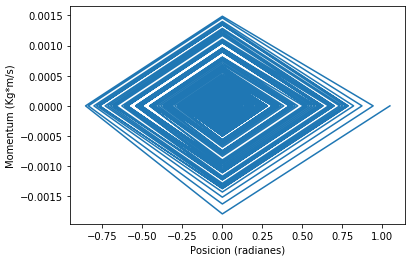
\includegraphics[width=8cm, height=7cm]
					{diagramaFase60.png}}	
				\c	aption{Diagrama de fase del p\'endulo simple a un \'angulo inicial de 60 grados.}
				\label{fig:DiagramaFase60}
			\end{figure} 
	
			\begin{figure}[!htb]
				\center{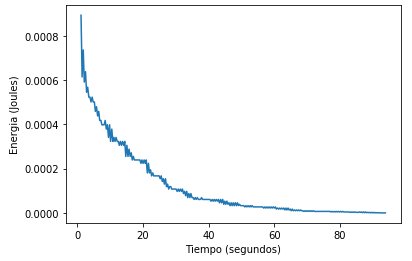
\includegraphics[width=8cm, height=7cm]
					{EnergiaTiempo60.png}}	
				\caption{Energ\'ia vs Tiempo del p\'endulo simple a un \'angulo inicial de 60 grados.}
				\label{fig:EnergiaTiempo60}
			\end{figure} 
	
	\section{An\'alisis y conclusiones}
		Una de las ecuaciones principales de este experimento recae en la ecuaci\'on (\ref{ecuacionMovimiento}). Con esta ecuaci\'on, en un principio, se tendr\'ia toda informaci\'on relevante de la din\'amica del p\'endulo. Esta ecuaci\'on toma la siguiente forma:
			\begin{equation}
				\ddot{\theta} + 2\beta\dot{\theta} + sen(\theta) = 0
				\label{movimientoReal}	
			\end{equation}  
		donde $2\beta$ es el factor que hace el movimiento amortiguado. El par\'ametro $\beta$ es igual a $b/2m$, siendo $b$ el factor de la fuerza no conservativa que amortigua la oscilaci\'on. La ecuac\'ion (\ref{movimientoReal}) no tiene soluci\'on anal\'itica y solo se puede aproximar el resultado por medio de m\'etodos num\'ericos. Se utiliz\'o el m\'etodo de Runge-Kutta de orden cuatro, para que la soluci\'on tenga mayor exactitud\cite{pang1999introduction}. La ecuaci\'on es: 
			\begin{equation}
				y_{i+1} = y_{i} + \frac{1}{6}(c_1 + 2c_2 + 2c_3 + c_4)
				\label{RKecuacion}	
			\end{equation} 
		siendo $y_1 = \theta$ y $y_2 = \dot{\theta}$. Antes de entrar en detalle de la soluci\'on num\'erica, se explica los datos obtenidos para cada \'angulo inicial.\\
		\indent La figura (\ref{fig:DiagramaFase60}) muestra el diagrama de fase del sistema cuando el \'angulo inicial es de 60 grados. El inicio del diagrama es cuando el momentum es cero y la posici\'on es maxima. Se dice que el periodo de una oscilaci\'on completa es igual al movimiento que va desde un \'angulo positivo con momentum cero al pr\'oximo \'angulo positivo con momentum cero. Lo interesante del diagrama es como el movimiento decae bruscamente en los primeros periodos. Este decaimiento brusco es resultado de las fuerzas no conservativas. Estas fuerzas ser\'ian solamente las fuerzas de fricci\'on. Hay fricci\'on en el pivote, en la cuerda con el protractor y la resistencia del aire. Entonces, el decaimiento brusco se debe al sistema mismo, tratando de perder la m\'inima energ\'ia posible. Las figuras (\ref{fig:DiagramaFase45}) y (\ref{fig:DiagramaFase30}) muestran un comportamiento similar a la figura (\ref{fig:DiagramaFase60}), por lo tanto se cumple lo antes mencionado.\\
		\indent En la gr\'afica (\ref{fig:EnergiaTiempo60}) se puede observar que el decaimiento de la energ\'ia es exponencial. Regresando a la ecuaci\'on (\ref{EcuacionHamilton}), que corresponde al Hamiltoniano dependiente del tiempo, se puede inferir entonces que $H^{(1)}$ tiene la forma de:
			\begin{equation}
				H^{(1)} = \epsilon H^{(0)};
			\end{equation}  
		donde
			\begin{equation}
		 		\epsilon = -(1 - e^{-\alpha t}).
			\end{equation} 
		As\'i $\epsilon\rightarrow0\Rightarrow H' = H^{(0)}$ y cuando $\epsilon\rightarrow\infty\Rightarrow H'\rightarrow0$. Por lo tanto, para saber el decaimiento de cualquier sistema similar, es solo cuesti\'on de ajustar $\alpha$ al valor que mejor se acomode a los resultados experimentales. Al comparar las gr\'aficas para los otros dos \'angulos (gr\'aficas \ref{fig:EnergiaTiempo45} y \ref{fig:EnergiaTiempo30}) el comportamiento es similar a excepci\'on de un mayor decaimiento de la energ\'ia cuando la energ\'ia inicial es mayor. Parece ser que la energ\'ia tiene mayor decaimiento dependiendo de sus condiciones iniciales del \'angulo. Esto podr\'ia ser resultado de lo antes mencionado, el sistema inicialmente pierde energ\'ia bruscamente porque est\'a acomodando su din\'amica para que durante el resto del movimiento se pierda la m\'inima energ\'ia posible. Tambi\'en podr\'ia ser que el factor de la fuerza disipativa $\beta$ sea diferente dependiendo el \'angulo inicial del sistema.\\
		\indent Volviendo a la soluci\'on n\'umerica de la ecuaci\'on (\ref{movimientoReal}) por el m\'etodo Runge-Kutta, las condiciones iniciales fueron: $\theta = 60\pi/180, 45\pi/180, 30\pi/180$ con $\dot{\theta} = 0, 0, 0$ donde cada coma indica el sistema independiente a sus condiciones iniciales. El diagrama de fase utilizando este m\'etodo esta dado en la figura (\ref{fig:RK60}). La raz\'on por la cual se ve como un sistema con disipaci\'on mas fuerte es debido a la cantidad de iteraciones. Con muchas iteraciones el comportamiento ser\'ia m\'as parecido al de la figura (\ref{fig:DiagramaFase60}). El p\'arametro $\beta$ es una variable din\'amica en este m\'etodo y es necesario darle el debido ajuste que exprese mejor los datos experimentales. Para los otros dos \'angulos, 45 y 30 grados, el diagrama de fase estan en las figuras (\ref{fig:RK45}) y (\ref{fig:RK30}), respectivamente. \\ 
		Se concluye que el sistema siempre trata de perder la m\'inima energ\'ia posible. Es decir, trata de acomodar su din\'amica para prolongar el movimiento el m\'aximo tiempo posible. Cumple el principio de m\'inima acci\'on. Adem\'as se encontr\'o que el sistema no es extrictamente ca\'otico matematicamente hablando pero si comparte ciertas caracter\'isticas de sistemas ca\'oticos.           
		   
		
		\begin{figure}[!htb]
			\center{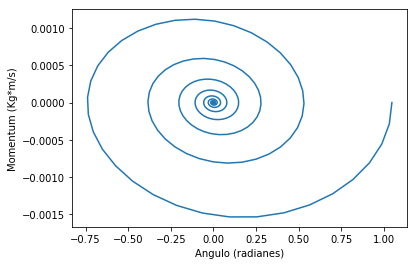
\includegraphics[width=8cm, height=7cm]
				{RK60.png}}	
			\caption{Soluci\'on de la ecuaci\'on (\ref{movimientoReal}) por el m\'etodo de Runge-Kutta para un \'angulo inicial de 60 grados.}
			\label{fig:RK60}
		\end{figure}   
		 
		 
	
%	\section{Agradecimientos}
	
	\section{Anexos}
	
		\begin{figure}[!htb]
			\center{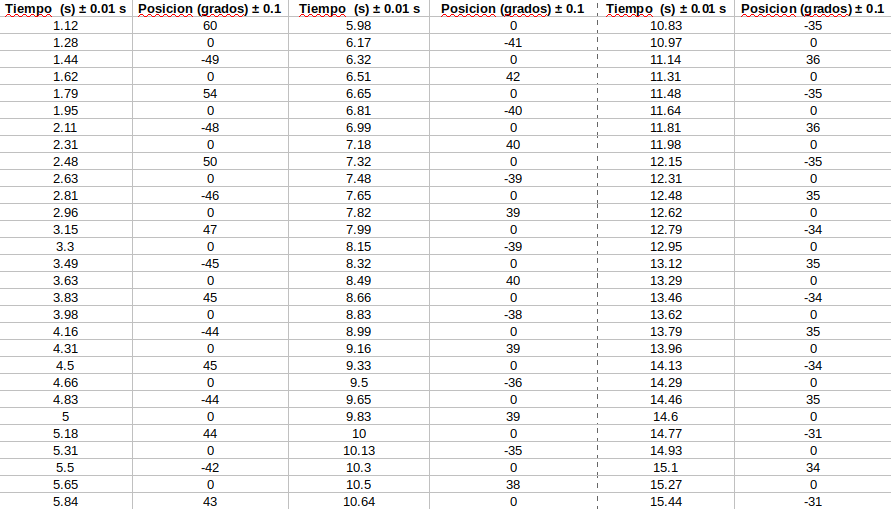
\includegraphics[width=8cm, height=7cm]
				{penduloSimple60.png}}
			\caption{Tabla de los primeros datos promedio de la posici\'on y el tiempo del pendulo simple a 60 grados inicialmente (a un cuarto de periodo cada toma).}
			\label{fig:penduloSimple60}
		\end{figure} 
		
		\begin{figure}[!htb]
			\center{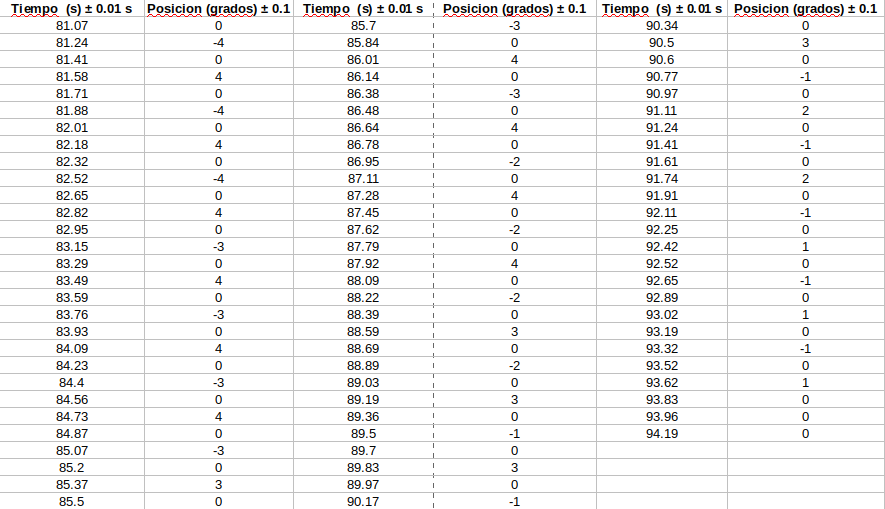
\includegraphics[width=8cm, height=7cm]
				{penduloSimple60B.png}}	
			\caption{Tabla de los \'ultimos datos del movimiento del pendulo simple a \'angulo inicial de 60 grados (a un cuarto de periodo cada toma).}
			\label{fig:penduloSimple60B}
		\end{figure} 
		
		\begin{figure}[!htb]
			\center{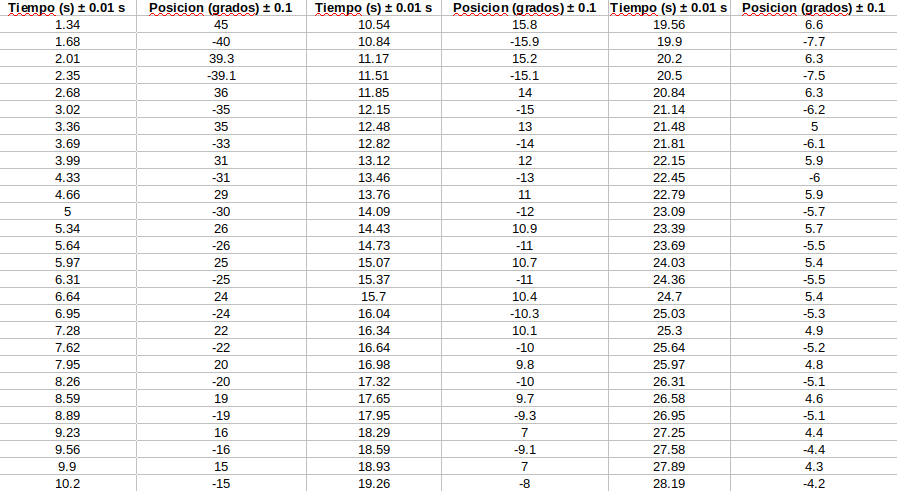
\includegraphics[width=8cm, height=7cm]
				{penduloSimple45.png}}	
			\caption{Tabla de los primeros datos del movimiento del p\'endulo simple a \'angulo inicial de 45 grados (a medio periodo cada toma).}
			\label{fig:penduloSimple45}
		\end{figure} 
		
		\begin{figure}[!htb]
			\center{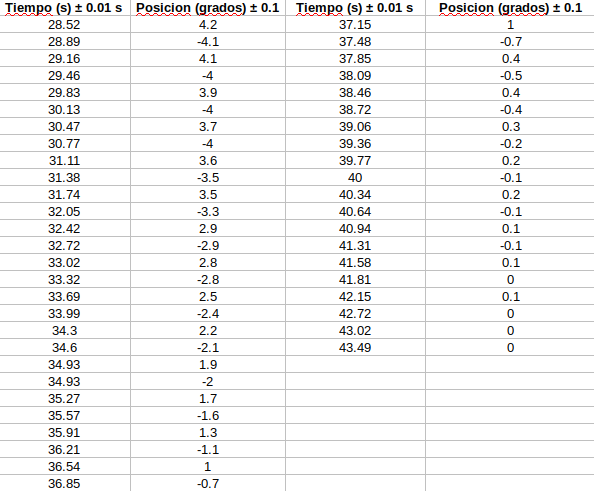
\includegraphics[width=8cm, height=7cm]
				{penduloSimple45B.png}}	
			\caption{Tabla de los \'ultimos datos del movimiento del p\'endulo simple a \'angulo inicial de 45 grados (a medio periodo cada toma).}
			\label{fig:penduloSimple45B}
		\end{figure} 
		
		\begin{figure}[!htb]
			\center{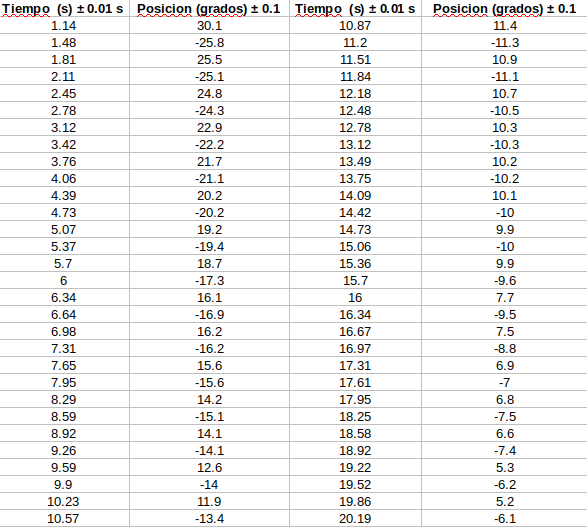
\includegraphics[width=8cm, height=7cm]
				{penduloSimple30.png}}	
			\caption{Tabla de los primeros datos del movimiento del pendulo simple a \'angulo inicial de 30 grados (a medio periodo cada toma).}
			\label{fig:penduloSimple30}
		\end{figure} 
		
		\begin{figure}[!htb]
			\center{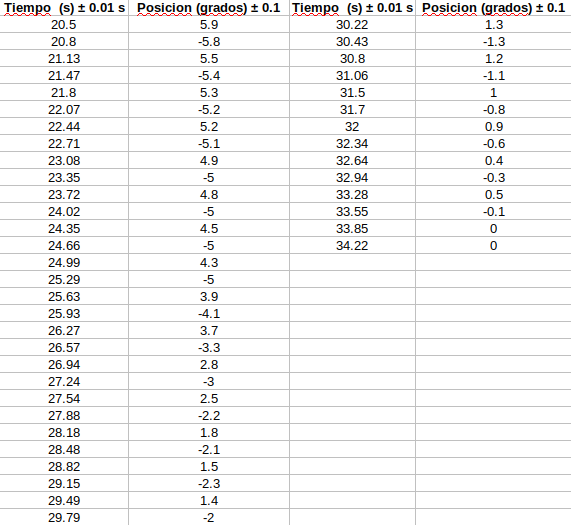
\includegraphics[width=8cm, height=7cm]
				{penduloSimple30B.png}}	
			\caption{Tabla de los \'ultimos datos del movimiento del p\'endulo simple a \'angulo inicial de 30 grados (a medio periodo cada toma).}
		\end{figure} 
	
		\begin{figure}[!htb]
			\center{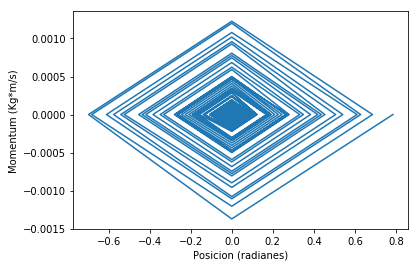
\includegraphics[width=8cm, height=7cm]
				{diagramaFase45.png}}	
			\caption{Diagrama de fase del p\'endulo simple a un \'angulo inicial de 45 grados.}
			\label{fig:DiagramaFase45}
		\end{figure} 	
		
		\begin{figure}[!htb]
			\center{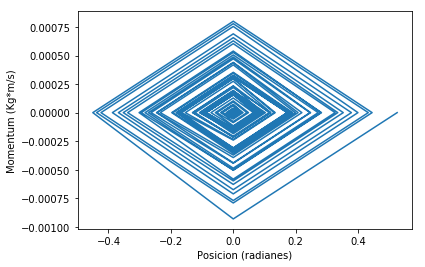
\includegraphics[width=8cm, height=7cm]
				{diagramaFase30.png}}	
			\caption{Diagrama de fase del p\'endulo simple a un \'angulo inicial de 30 grados.}
			\label{fig:DiagramaFase30}
		\end{figure} 
	
		\begin{figure}[!htb]
			\center{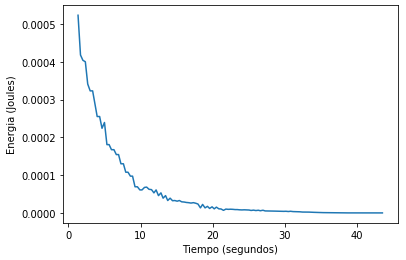
\includegraphics[width=8cm, height=7cm]
				{EnergiaTiempo45.png}}	
			\caption{Energ\'ia vs Tiempo del p\'endulo simple a un \'angulo inicial de 45 grados.}
			\label{fig:EnergiaTiempo45}
		\end{figure} 
		
		\begin{figure}[!htb]
			\center{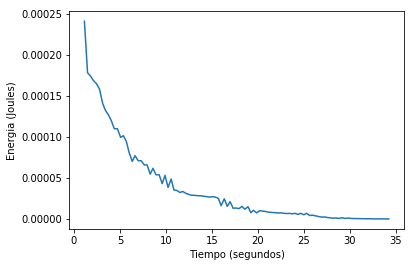
\includegraphics[width=8cm, height=7cm]
				{EnergiaTiempo30.png}}	
			\caption{Energ\'ia vs Tiempo del p\'endulo simple a un \'angulo inicial de 30 grados.}
			\label{fig:EnergiaTiempo30}
		\end{figure}
	
		\begin{figure}[!htb]
			\center{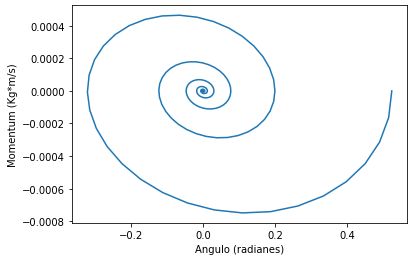
\includegraphics[width=8cm, height=7cm]
				{RK30.png}}	
			\caption{Soluci\'on de la ecuaci\'on (\ref{movimientoReal}) por el m\'etodo de Runge-Kutta para un \'angulo inicial de 30 grados.}
			\label{fig:RK30}
		\end{figure}
	  
		\begin{figure}[!htb]
			\center{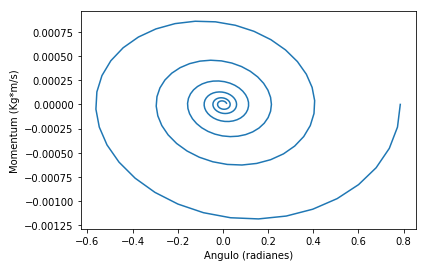
\includegraphics[width=8cm, height=7cm]
				{RK45.png}}	
			\caption{Soluci\'on de la ecuaci\'on (\ref{movimientoReal}) por el m\'etodo de Runge-Kutta para un \'angulo inicial de 45 grados.}
			\label{fig:RK45}
		\end{figure} 
		
		\begin{figure}[!htb]
			\center{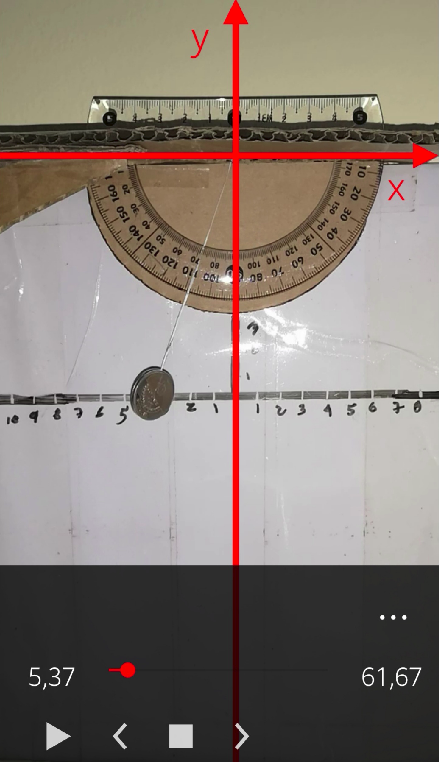
\includegraphics[width=8cm, height=13cm]
				{equipoPendulo.png}}	
			\caption{Foto del equipo. Se puede ver como se estudi\'o el movimiento a la hora de tomar datos. La posici\'on de la masa es a 19.1 grados con un tiempo de 5,37 segundos}
			\label{fig:equipo}
		\end{figure} 
		
		%\begin{tabular}{ |p{3cm}||p{3cm}|p{3cm}|p{3cm}|  }
			%\hline
			%\multicolumn{4}{|c|}{\colorbox{BurntOrange}{\textbf{Cronograma}}} \\
			%\hline
			%Fechas importantes& 13 al 27 (abril) &27 (abril) al 15 (junio)&15 al 29 (junio)\\
			%\hline
			%Armar equipo &\centering \checkmark  &\centering \checkmark  &   \\
			%Toma de datos&& \centering\checkmark&\\
			%An\'alisis de datos & &\centering\checkmark&\checkmark\\
			%Programar c\'odigo& &\centering\checkmark& \checkmark \\
			%Presentaci\'on&     & &\checkmark\\
			%Poster&   &    &\checkmark\\
			%Primer avance&  \centering\checkmark  &    &\\
			
			%\hline
		%\end{tabular}
	
		\bibliographystyle{abbrv}
		\bibliography{MyReference.bib}
	
	
\end{document}